\documentclass[11pt]{article}
\usepackage[utf8]{inputenc} % Para caracteres en espa�ol
\usepackage{amsmath,amsthm,amsfonts,amssymb,amscd}
\usepackage{multirow,booktabs}
\usepackage[table]{xcolor}
\usepackage{fullpage}
\usepackage{lastpage}
\usepackage{enumitem}
\usepackage{multicol}
\usepackage{fancyhdr}
\usepackage{mathrsfs}
\usepackage{wrapfig}
\usepackage{setspace}
\usepackage{esvect}
\usepackage{calc}
\usepackage{multicol}
\usepackage{cancel}
\usepackage{graphicx}
\graphicspath{ {pictures/} }
\usepackage[retainorgcmds]{IEEEtrantools}
\usepackage[margin=3cm]{geometry}
\usepackage{amsmath}
\newlength{\tabcont}
\setlength{\parindent}{0.0in}
\setlength{\parskip}{0.05in}
\usepackage{empheq}
\usepackage{framed}
\usepackage{newtxmath}
\usepackage{euscript}
\DeclareMathAlphabet{\mathpzc}{T1}{pzc}{m}{it}
\usepackage[most]{tcolorbox}
\usepackage{xcolor}
\colorlet{shadecolor}{orange!15}
\parindent 0in
\parskip 12pt
\geometry{margin=1in, headsep=0.25in}
\theoremstyle{definition}
\newtheorem{defn}{Definition}
\newtheorem{reg}{Rule}
\newtheorem{exer}{Exercise}
\newtheorem{note}{Note}
\newcommand{\volume}{{\ooalign{\hfil$V$\hfil\cr\kern0.08em--\hfil\cr}}}
\newcommand{\parr}{\mathbin{\|}} % Parralel Symbol
\begin{document}
\setcounter{section}{0} %Section before the section you want. I want section 1 I put 0
\setcounter{page}{3} %page number you want to be the first page
\setcounter{equation}{1} %equation before the equation you want I want equation 2 I put 1
%\definecolor{babyblue}{rgb}{0.54, 0.81, 0.94}
\definecolor{babyblueeyes}{rgb}{0.63, 0.79, 0.95}
\definecolor{babyblue}{rgb}{0.69, 0.88, 0.9}

 \pagestyle{fancy}
 
\fancyhf{}
\rhead{Section 5:  Collisions}
\rfoot{Page \thepage}
\thispagestyle{empty}


\begin{center}
{\LARGE \bf Section 5:  Collisions}\\
{\large AE435}\\
Spring 2018
\end{center}
\vspace{5mm}
\section{Cross Sections}
The collision "cross-section" is like the target size a particle "sees" as it moves through a collection of particles.
 
Some cross-sections tell us how (to what angle) the incident particle will be scattered due to a particle type of collision, these are "differential cross-sections".
 
If we integrate the differential cross-section over all possible scatter angles you get the "total" or "effective" cross-section for that particular type of collision.
 
Finally, if you sum the effective (or total) cross-section for all possible collision types, you get the "total" collision cross-section.
\tableofcontents
\newpage
\subsection{Effective Cross Sections}
Consider
\begin{itemize}
\item A particle of type j encountering
\item A particle of type k
\item In collision of type $\beta$
\end{itemize}
 
The probability of this over a path length  $\mathrm{d}x$   is:
\begin{shaded}
\textbf{Probability of Encounter}
\begin{equation}
\begin{aligned}
\mathrm{d}P_{jk}^{(\beta)} = n_k \, Q_{jk}^{(\beta)} \, \mathrm{d}x
\end{aligned}
\end{equation}
Where
\begin{equation*}
\begin{aligned}
Q_{jk}^{(\beta)} &= \text{Corresponding Collision Cross-Section} \\
&= [m^{-3} \,m^{2} \,m^{1}] = [1] \quad \text{Unitless}\\
\end{aligned}
\end{equation*}
\end{shaded}
 
 For a flux ($\Gamma$) of test particles, j, entering a cloud of field particles, k, the flux leaving the cloud is:
 \begin{center}
\vfill
\begin{equation}
\begin{aligned}
\Gamma + \mathrm{d}\Gamma = \Gamma\big(1-\mathrm{d}P_{jk}^{(\beta)}\big) = \Gamma\big(1-n_k \, Q_{jk}^{(\beta)} \, \mathrm{d}x \big)
\end{aligned}
\end{equation}

\textbf{Figure 3}
\end{center}
\newpage
Cancelling like terms yields:
 \begin{equation}
\begin{aligned}
\mathrm{d}\Gamma = \Gamma \, n_k \, Q_{jk}^{(\beta)} \, \mathrm{d}x \big)
\end{aligned}
\end{equation}

Which integrates to:
\begin{equation}
\begin{aligned}
\Gamma =\Gamma_o \, \exp \bigg(-n_k \, Q_{jk}^{(\beta)} \, x \bigg) = \Gamma_o \, \exp \Bigg(-\frac{x}{\lambda_{\text{mfp}}}\Bigg)
\end{aligned}
\end{equation}

where $\Gamma_o$ is the initial flux. The mean free path now becomes
\begin{equation}
\begin{aligned}
\lambda_{\text{mfp}} = \frac{1}{n_k \, Q_{jk}^{(\beta)}}
\end{aligned}
\end{equation}

A good first estimate for          $Q_{jk}^{(\beta)}$  	is the... atomic cross section
\begin{shaded}
\textbf{Atomic Cross Section}
\begin{equation}
\begin{aligned}
a_o = \frac{\epsilon_o \, h^2}{\pi \, m_e \, q_e^2}
\end{aligned}
\end{equation}

Where the Bohr radius $\pi a_o^2$ describes the orbit for an electron with the lowest possible non-zero momentum.
\end{shaded}
 
Returning to the collisional cross-section, note that
 
\begin{equation}
\begin{aligned}
Q_{jk}^{(\beta)} = Q_{kj}^{(\beta)}
\end{aligned}
\end{equation}
We can define a...
\begin{shaded}
\textbf{Total ("Effective") Cross-Section}
\begin{equation}
\begin{aligned}
Q_{jk} = \sum_{\beta} \, Q_{jk}^{(\beta)}
\end{aligned}
\end{equation}
which is the sum of all the different types of collisions (elastic, excitation, ionization, etc.).
\end{shaded}
\newpage
\subsection{Differential Cross-Sections}
In addition to Effective Cross Sections, we also have differential cross-sections $q(\theta)$ defined by the scattering angle,
\begin{center}
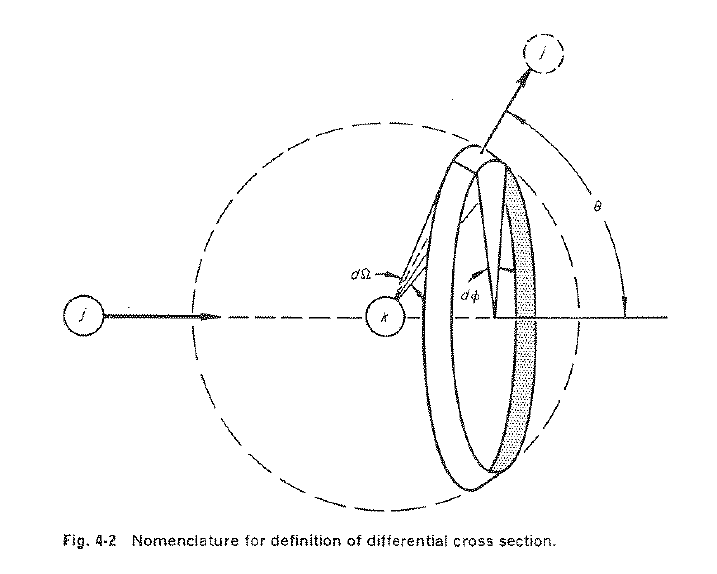
\includegraphics[scale=.45]{1.png}
\end{center}
The probability of scattered particle emerging into solid angle:
 \begin{equation}
\begin{aligned}
\mathrm{d}\Omega = \sin\theta \, \mathrm{d}\theta \, \mathrm{d}\phi
\end{aligned}
\end{equation}
is
 \begin{equation}
\begin{aligned}
\mathrm{d}P(\theta) = q(\theta) \, \mathrm{d}\Omega = q(\theta) \, \sin\theta \, \mathrm{d}\theta \, \mathrm{d}\phi
\end{aligned}
\end{equation}

Integrating over the full $4\pi$ of the solid angle around the scattering center gives us the:
 \begin{shaded}
 \textbf{Total Collisional Cross-Section}
  \begin{equation}
\begin{aligned}
Q = \int_{0}^{2\pi} \int_{0}^{\pi} \, q(\theta) \, \sin\theta \, \mathrm{d}\theta \, \mathrm{d}\phi
\end{aligned}
\end{equation}
 \end{shaded}
For a type $-\beta$ collision, the mean free path is
  \begin{equation}
\begin{aligned}
\lambda_{\text{mfp}}^{(\beta)} = \frac{1}{n_k \, Q_{jk}^{(\beta)}}
\end{aligned}
\end{equation}

as previously defined in Equation 6 and Equation 4.15
 
We can now define...
 
 \begin{shaded}
\textbf{Collision Frequency}
\begin{equation}
\begin{aligned}
\nu_{jk}^{(\beta)} = n_k \, Q_{jk}^{(\beta)} \, \overline{v_{jk}}
\end{aligned}
\end{equation}
Where
\begin{equation*}
\begin{aligned}
\overline{v_{jk}} &= \text{Collision Speed}
&=  \text{Relative Speed Between j and k}
\end{aligned}
\end{equation*}
\end{shaded}
The collision speed $\overline{v_{jk}}$ is well-defined in beam experiments, but less so for thermal plasmas. 

\begin{framed}
\textbf{General Equation for Collision Speed in Thermal Plasmas:}
\begin{equation}
\begin{aligned}
\overline{v_{jk}} \cong v_{th} = \Bigg(\frac{8 \, k \, T}{\pi \, m}\Bigg)^{\frac{1}{2}} \qquad \qquad \text{Equation 4.32}
\end{aligned}
\end{equation}
This relation applies for the faster particle species in mixed thermal plasmas.  

\textbf{Example:} Consider a xenon plasma with equal electron and ion temperature ($T_e = T_i = 3$eV).

As a result...   
\begin{equation*}
\begin{aligned}
\left\{\begin{matrix}
V_e = 750 \, \frac{km}{s}
\\ 
V_i = 1.5 \, \frac{km}{s}
\end{matrix}\right.
\end{aligned}
\end{equation*}

Meaning that...
\begin{equation*}
\begin{aligned}
\nu &= n \, <Q_{jk} \, V_{jk}> \\
&= n \, \overline{Q_{jk} \, V_{jk}}
\end{aligned}
\end{equation*}

Such that
\begin{equation*}
\begin{aligned}
\overline{Q \, V} = \int_{0}^{\infty} \, Q \, v \, f(v) \, \mathrm{d}v
\end{aligned}
\end{equation*}
\end{framed}

Finally, can define a:
\begin{shaded}
\textbf{Mean Collision Rate for a Swarm of Particles}
\begin{equation}
\begin{aligned}
\nu_{jk}^{(\beta)} = n_k \, Q_{jk}^{(\beta)} \, \overline{v_{jk}}
\end{aligned}
\end{equation}
Where
%\begin{equation*}
%\begin{aligned}
%\end{aligned}
%\end{equation*}
\begin{itemize}
\item We can approximate      	and         	as Maxwellians,
\item shows the dependence of Q on relative velocity.
\end{itemize}
\end{shaded}
\end{document}